\begin{frame}\frametitle{Tracing simulation}
Simgrid despose of a visualization tracing model that works through gathering data about the resource of links and hosts of a turned simulation whatever the interface (MSG, SimDag, SMPI, and S4U).\\

%The idea of the tracing facilities is to give SimGrid users to possibility to classify MSG and SimDAG tasks by category. \\
\begin{exampleblock}{Tracing before}
The previous model was written under C code in such way it emulate the CPP OOP.
\end{exampleblock}
%This latter mean that any task is not classified according to a category is not traced. If no categories are specified, simulations can still be traced using a special parameter in the command line.

%This means that the tracing will register how much power is used for each host and how much bandwidth is used for each link of the platform.
\end{frame}
\begin{frame}\frametitle{Tracing after}
\begin{exampleblock}{}
We were able to make some several improvements on the code 
\begin{itemize}
\item Remove the useless structures and functions.
\item Make an hierarchical class tree that are shown in the below figure.
\end{itemize}
\end{exampleblock}
\begin{figure}
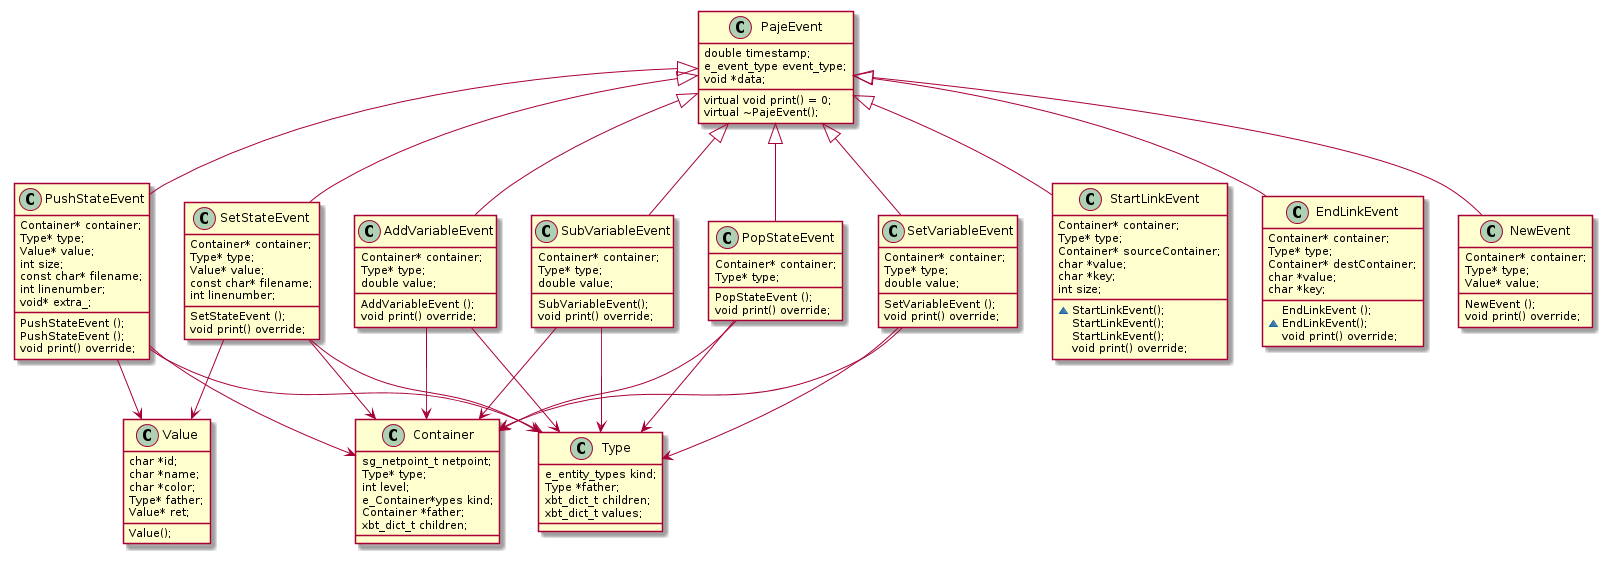
\includegraphics[width=10.5cm]{figures/diagram_simgrid.png}
\end{figure}
\end{frame}